\subsection{Was ist Deployment}

Wenn man vom Deployment spricht meint man die Bereitstellung von Software. Dies erfolgt alles über automatisierte Prozesse, mittels derer die Installation und Konfiguration der Softwarelösungen erfolgt. Im Deployment sind Aspekte wie die Installation, Konfiguration Aktualisierung und Wartung von Systemene enthalten.
\cite{Deployment}


\subsection{Verschiedene Arten von Deployment}

Grundsätzlich gibt es verschiedene Arten von Deployment. Diese werden prinzipell folgendermaßen kategorisiert:
    \begin{itemize}
    \item Traditionelles Deployment
    \item Virtuelles Depoyment
    \item Container Deployment
    \end{itemize}

\subsection{Traditionelles Deployment}

Früher wurde eine Anwendung auf einem physischen Server deployed. Damals sah das ganze folgendermaßen aus:

\begin{itemize}
    \item Einen Server aufsetzen
    \item Ein Betriebssystem auf dem Server installieren
    \item Auf dem Server benötigte Tools wie z.B Node oder NPM installieren
    \item Die benötigten Dateien auf den Server kopieren
    \item Die Anwendung laufen lassen
\end{itemize}

Solange nur eine einzige Anwendung auf diesem Server läuft, stellt dies kein Problem dar. Sogar im Gegenteil die Anwendung läuft dann sehr performant auf dem Server, da er jegliche Ressourcen die der Server frei hat benutzt. Sobald dann aber mehr als nur eine Anwendung auf einem Server laufen, führt dies zu Problemen, diese können sein:

\begin{itemize}
    \item Fehlende Ressourcen
    \item Dateninkonsistenzen durch gemeinsam genutzten Speicher
    \item Hacker Attacken
\end{itemize}


\cite{Verschiedene_Deployment_Arten}    


\subsection{Virtuelles Deployment}

Um die Probleme gemeinsam genutzter Speicher zu lösen und die Skalierbarkeit zu verbessern, begann die Virtualisierung. In diesem Fall wurde eine virtuelle Maschine erstellt, die über ihre eigene Partition im Speicher und ein eigenes Betriebssystem verfügte. Dies ermöglichte die gewünschte Isolierung der Anwendungen und eine bessere Aufteilung der verfügbaren Ressourcen. Dennoch traten auch einige Probleme bei dieser Lösung auf, darunter:

\begin{itemize}
\item Die Größe und der Overhead des Betriebssystems.
\item  Lange Startzeiten.
\item  Mangelnde Skalierbarkeit der Anwendungen.
\end{itemize}

\cite{Virtuelles_Deployment}

\subsection{Container Deployment}

\begin{figure}
    \centering
    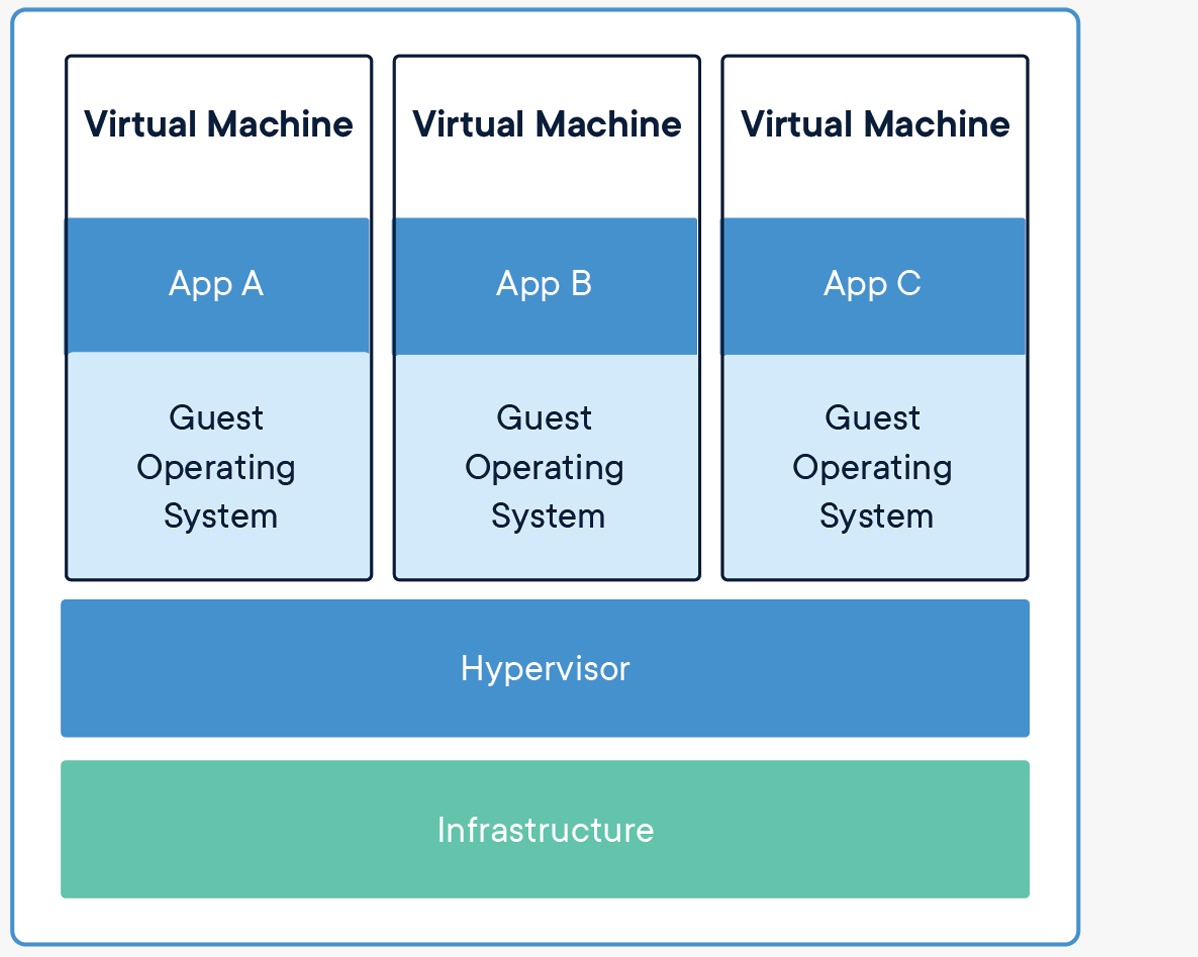
\includegraphics[width=0.8\linewidth]{pics/container_deployment.jpeg}
    \caption{Container Deployment}
    \label{fig:enter-label}
\end{figure}


Container sind in sich geschlossene, autarke Einheiten, die sämtlichen Anwendungscode und sämtliche erforderlichen Abhängigkeiten in sich tragen. Neben Docker, einem der prominentesten Werkzeuge zur Containerisierung von Anwendungen, stehen auch Alternativen zur Verfügung, darunter Lösungen wie Kubernetes und Podman.

\subsubsection{Vorgang des Container Deployments}

Als erstes wird die gesamte Anwendung in ein Container Image verpackt. In diesem Image befindet sich der Anwendungscode, die Laufzeitumgebung und alle erforderlichen Abhängigkeiten wie zum Beipsiel Node oder NPM.

Als nächstes wird das erstellte Container Image in einem Container-Image-Repository wie Docker Hub registriert und gespeichert.

Danach müssen die Container Images bereitgestellt werden dies geschieht überlicherweise auf einem Container-Orchestrierungs-Framework wie Kubernetes oder Docker Swarm.

Als letzten Schritt muss der Container noch konfiguriert werden und mögliche Umgebungsvariablen gesetzt werden.

Wenn eine neue Version der Anwendung verfügbar ist, kann das Container-Deployment-Framework verwendet werden, um die Container schrittweise zu aktualisieren, ohne die Verfügbarkeit der Anwendung zu beeinträchtigen.

\subsection{Umgebungsvariablen}

Umgebungsvariablen sind dazu da um die Anwendungsgeheimnisse und Konfigurationen zu speichern, die wenn nötig von der Anwendung abgerufen werden können. Umgebungsvariablen verleihen einer Anwendung mehr Dynamik. Somit kann von sehr schnell und einfach von internen auf externe Ressourcen umgeschaltet werden.

\subsubsection{.env-Dateien}

Eine der einfachsten Methoden um eine Umgebungsvariable zu speichern sind .env-Dateien. Hierbei wird das .env File einfach auf Top-Level des Repository gespeichert und somit können in dieser Datei dann beliebig viele Umgebungsvariablen gespeichert werden.

\begin{verbatim}
    VAR_UNO=SOME_KEY_HERE
    VAR_DOS=SOME_OTHER_KEY_HERE
\end{verbatim}

\cite{Umgebungsvariablen}



\subsection{Docker}

Docker wurde erstmals im März 2013 von dotCloud veröffentlicht und nutzt den Linux-Kernel und seine Ressourcenkontrollmechanismen wie Cgroups und Namespaces, um Prozesse zu isolieren, wodurch sie in voneinander unabhängigen Umgebungen ausgeführt werden können. Dieser fundamentale Aspekt der Container-Technologie ermöglicht die parallele Ausführung mehrerer Prozesse und Anwendungen in isolierten Containern. Dies steigert die Effizienz Ihrer Infrastruktur, ohne dabei die Sicherheitsvorteile zu vernachlässigen, die sich aus der Nutzung separater Umgebungen ergeben.

Container-Tools wie zum Beispiel Docker arbeiten auf mit einem imagebasierten Deployment-Modell. Dies erleichtert der Anwendung die Nutzung von gemeinsamen Ressourcen und Services mit sämtlichen Abhängigkeiten.

Mit Docker ist es möglich einen Teil einer Anwendung zu aktualisieren oder reparieren ohne die gesamte Anwendung deaktivieren zu müssen. Außerdem besitzt Docker eine Rollbacking, also das zurücksetzen auf die vorherige Version.

\cite{Vorteile_Nachteile_Docker}
\cite{Was_ist_Docker}




